\documentclass[a4paper,onecolumn, 10pt]{article}
\usepackage[utf8]{inputenc}
\usepackage[portuguese,brazil]{babel}
\usepackage{ae}

\usepackage[pdftex]{graphicx} % Exposta para pdf e aceita figuras
%\usepackage{indentfirst} % Identa primeiro paragrafo
\usepackage{textcomp}
\usepackage[margin=30mm]{geometry}
\usepackage[pdfauthor={Pedro Rosanes},% Insere metadados com o nome do autor
	    pdftitle={Extensão dos mecanismos de gerência de tarefas do sistema operacional TinyOS},% Título que será mostrado na janela do PDF
	    pdftex]{hyperref} % Usa hiperlinks no decorrer do texto
%\parskip 7.2pt           % sets spacing between paragraphs
\renewcommand{\baselinestretch}{1.5}

\usepackage{color}
\usepackage{listings}
\lstset{ %
language=C++,                % choose the language of the code
basicstyle=\footnotesize,       % the size of the fonts that are used for the code
backgroundcolor=\color{white},  % choose the background color. You must add
showspaces=false,               % show spaces adding particular underscores
showstringspaces=false,         % underline spaces within strings
showtabs=false,                 % show tabs within strings adding particular underscores
frame=single,                   % adds a frame around the code
tabsize=2,                  % sets default tabsize to 2 spaces
captionpos=b,                   % sets the caption-position to bottom
breaklines=true,                % sets automatic line breaking
breakatwhitespace=false,        % sets if automatic breaks should only happen at whitespace
title=\lstname,                 % show the filename of files included with \lstinputlisting;
% also try caption instead of title
escapeinside={\%*}{*)},         % if you want to add a comment within your code
morekeywords={*,...},            % if you want to add more keywords to the set
belowskip=0pt
}

%---------------------------------------------------------------------------------------------------
\title{Extensão dos mecanismos de gerência de tarefas do sistema operacional TinyOS}
\author{Bolsista: Pedro Rosanes \and Orientador: Silvana Rossetto \and Departamento de Ciência da Computação}
\date{11 de abril de 2011}

\begin{document}

%\begin{titlepage}
\maketitle
%\tableofcontents
%\end{titlepage}

\abstract{Resumo}\label{resumo}
Redes de Sensores Sem Fio (RSSFs) são formadas por pequenos dispositivos de sensoreamento, com 
espaço de memória e capacidade de processamento limitados, fonte de energia esgotável e comunicação sem fio.
O sistema operacional mais usado na programação desses dispositivos é o TinyOS, um sistema leve, 
projetado especialmente para consumir pouca energia, um dos requisitos mais importante para RSSFs. 
%O modelo  programação adotado pelo TinyOS é orientada a componentes (para facilitar a
%reutilização de código) e basedo em eventos (para economizar memória), 
O modelo de programação adotado pelo TinyOS prioriza o atendimento de interrupções.
Em função disso, as operações são normalmente divididas em duas fases: uma para envio
do comando, e outra para o tratamento da resposta (evento sinalizado via interrupção). 
Esse modelo de programação, baseado em eventos, quebra o fluxo de execução normal, dificultando a
tarefa dos desenvolvedores de aplicações. 
Para que os tratadores de eventos (interrupções) sejam curtos, tarefas maiores são
postergadas para execução futura e, para evitar concorrência entre elas,
as tarefas são executadas em sequência, uma após a outra (i.e., uma tarefa só é iniciada após a tarefa
anterior ser concluída).  
O objetivo deste trabalho é propor e implementar políticas alternativas de escalonamento de tarefas
para o TinyOS visando a construção de abstrações de programação de nível mais alto que 
facilitem o desenvolvimento de aplicações nessa área.

%----------------------------------------------------------------------------------------------------
\section{Introdução}\label{intro}
Redes de Sensores Sem Fio (RSSFs) caracterizam-se pela formação de aglomerados de pequenos 
dispositivos que, atuando em conjunto, permitem monitorar ambientes físicos ou processos de 
produção com elevado grau de precisão. O desenvolvimento de aplicações que permitam explorar 
o uso dessas redes requer o estudo e a experimentação de protocolos, algoritmos e modelos de 
programação que se adequem às suas características e exigências particulares, entre elas, uso
de recursos limitados, adaptação dinâmica das aplicações, e a necessidade de integração com
outras redes, como a Internet.

Sistemas projetados para os dispositivos que formam as redes de sensores devem lidar apropriadamente
com as restrições e características particulares desses ambientes. 
A arquitetura adotada pelo TinyOS~\cite{tinyos/00} --- um dos sistemas operacionais mais usados
na pesquisa nessa área --- prioriza fortemente o tratamento dessas restrições em 
detrimento da simplicidade oferecida para o desenvolvimento de aplicações. 
A linguagem de programação usada é o nesC~\cite{nesc/03}, uma adaptação de C que provê baixo 
consumo de memória, optimizações, e previne condições de corrida.
Para lidar com as diversas operações de entrada e saída, o TinyOS utiliza um modelo de 
execução em duas fases, evitando bloqueios e consequentemente armazenamento de estados. 
A primeira fase da operação é um comando que pede ao hardware a execução de um serviço 
(ex.: sensoreamento). Este comando retorna imediatamente dando continuidade à execução. Quando o
serviço é terminado, o hardware envia uma interrupção, sinalizada como um evento pelo TinyOS. 
Então, o tratador do envento recebe as informações (ex., valor sensoreado) e lida com elas conforme programado. 
O problema gerado por essa abordagem é a falta da visão de um fluxo contínuo de execução 
na perspectiva do programador. 

O modelo de concorrência divide o código em dois tipos: assíncrono e síncrono. 
Um código  assíncrono pode ser alcançável a partir de pelo menos
um tratador de interrupção. Em função disso, a execução desses trechos do programa pode ser interrompida
a qualquer momento e é necessário tratar possíveis condições de corrida.
Um código síncrono é alcançável somente a partir de tarefas (\textit{tasks}) que são 
procedimentos adiados (postergados). Tarefas executam até terminar (não existe concorrência entre elas), 
por isso as condições de corrida são evitadas.  
As tarefas são todas escalonadas por um componente do TinyOS que usa uma política de escalonamento 
do tipo \textit{First-in First-out}~\cite{LevisGay/09}.

Com o objetivo de oferecer maior flexibilidade aos desenvolvedores de aplicações, 
a versão mais atual do TinyOS (versão 2.1.x) trouxe novas facilidades.
Uma delas é a possibilidade de substituir o componente de escalonamento de tarefas
para implementar diferentes políticas de escalonamento~\cite{TEP106}.
A outra é a possibilidade de usar o modelo de programação multithreading,
um modelo de programação mais conhecido pelos desenvolvedores de aplicações e que pode
ser usado como alternativa para lidar com as dificuldades do modelo de programação baseado em eventos.

Neste trabalho avaliamos essas novas facilidades do TinyOS.
Começamos propondo novos escalonadores de tarefas, implementando políticas de escalonamento por
prioridade. Avaliamos o modelo de multithreading oferecido, comparando diferentes formas de implementação
de uma aplicação básica e o custo da gerência de threads. O próximo passo será a implementação
de um mecanismo que permita gerência cooperativa de tarefas para o TinyOS, visando 
uma solução alternativa entre o modelo de escalonamento de tarefas que executam até terminar 
(e evitam condições de corrida) e o modelo de execução alternada entre as tarefas 
(que permite maior flexibilidade durante a execução, mas com custo de gerência alto).
Neste documento, apresentamos as atividades já executadas e os resultados alcançados.

%----------------------------------------------------------------------------------------------------
\section{Objetivos}\label{objetivos}
Os principais objetivos deste trabalho são:
\begin{itemize}
\item aprofundar o conhecimento sobre o modelo de concorrência do TinyOS;
\item avaliar as novas facilidades introduzidas na versão 2.1.x do TinyOS, 
incluindo a possibilidade de alterar o componente de escalonamento de tarefas e a implementação de threads;
\item propor e desenvolver diferentes políticas de escalonamento de tarefas;
\item implementar um mecanismo de gerência cooperativa de tarefas para o TinyOS baseado no 
conceito de co-rotinas~\cite{Rossetto/06}.
\end{itemize}

%----------------------------------------------------------------------------------------------------
\section{Metodologia}\label{metodologia}
Dividimos o trabalho em quatro etapas e dentro de cada etapa enumeramos as atividades
a serem desenvolvidas: 
\begin{enumerate}
\item {\bf Primeira etapa} %(out, nov)
\begin{itemize}
  \item Estudar material introdutório sobre as ferramentas TinyOS, nesC e TOSSIM (simulador do TinyOS).
  \item Instalar as ferramentas e experimentá-las em aplicações básicas.
  \item Estudar/revisar conceitos fundamentais sobre concorrência e gerência de tarefas em sistemas operacionais.
\end{itemize}
\item {\bf Segunda etapa} %(nov, dez, jan)
\begin{itemize}
  \item Estudar o modelo de concorrência do TinyOS.
  \item Projetar, implementar e avaliar outros componentes básicos de escalonamento de
  tarefas para o TinyOS.
  \item Redigir relatório técnico sobre os componentes de escalonamento desenvolvidos.
  \item Estudar o modelo de threads do TinyOS.
  \item Implementar aplicações básicas usando o modelo de threads do TinyOS.
  \item Redigir relatório técnico sobre o modelo de concorrência e os mecanismos de gerência de tarefas do TinyOS.
\end{itemize}
\item {\bf Terceira etapa} %(fev, mar, abr, mai)
\begin{itemize}
  \item Estudar o conceito de co-rotinas (mecanismo de gerência cooperativa de tarefas)
  \item Elaborar uma proposta de extensão do modelo de concorrência do TinyOS e
  dos seus mecanismos de gerência de tarefas.
  %\item Descrever resumidamente a proposta
  \item Projetar a solução e os experimentos que deverão ser realizados.
  %\item Descrever o projeto e modelagem da solução e dos experimentos
  \item Implementar a solução, executar os experimentos e avaliar os resultados.
  \item Redigir texto com proposta, projeto, modelagem, implementação e experiemntos  realizados.
\end{itemize}
\item {\bf Quarta etapa} %(mai, jun, jul, ago)
\begin{itemize}
%  \item Avaliar os resultados obtidos e refinar a proposta de solução.
  \item Propor trabalhos futuros.
%  \item Redigir relatório final sobre a Iniciação Científica: atividades realizadas, conhecimentos adquiridos, dificuldades encontradas.
  \item Redigir relatório técnico completo sobre o trabalho realizado. 
\end{itemize}
\end{enumerate}

%----------------------------------------------------------------------------------------------------
\section{Atividades realizadas}\label{atividades}
A seguintes atividades já foram realizadas:
\begin{itemize}
\item {\bf Estudo sobre o sistema operacional TinyOS}:
Estudo feito sobre o sistema operacional TinyOS, sua linguagem de programação nesC e o simulador TOSSIM.
Como fonte do aprendizado foram usados o minicurso desenvolvido pela 
professora Silvana Rosseto\cite{Rossetto/10}, o material oferecido
pela página do TinyOS\cite{tinyos}, e o livro \textit{TinyOS Programming}, de Levis e Gay\cite{LevisGay/09}.

\item {\bf Estudo sobre concorrência e gerência de tarefas em Sistemas Operacionais}:
Antes de estudar o modelo de concorrência e gerência de tarefas específica do TinyOS, 
foi feita uma revisão desses conceitas em sistemas operacionais em geral. 
O material utilizado foi o livro do professor Carlos Maziero (PUCPR)~\cite{Maziero/11}.

\item {\bf Estudo sobre concorrência e gerência de tarefas no TinyOS}:
Nessa etapa estudados o modelo de concorrência e os mecanismos de gerência 
de tarefas específicos do TinyOS, incluindo a sequência de inicialização do
TinyOS e o funcionamento do escalonador padrão.

\item {\bf Implementação de novos componentes de escalonamento de tarefas para o TinyOS}:
Após os estudos realizados, projetamos e desenvolvemos diferentes políticas de escalonamento
de tarefas para o TinyOS.

\item {\bf Estudo sobre o modelo de multithreading do TinyOS}:
Nessa etapa, estudamos o funcionamento do modelo de multithreading oferecido pela nova versão do TinyOS.

\item{\bf Estudo sobre a implementação de co-rotinas no TinyOS}:
Iniciamos o estudo sobre o conceito de co-rotinas, suas características básicas  e como ele 
pode ser  aplicado no TinyOS. Revisamos a implementação de co-rotinas proposta para a antiga versão do 
TinyOS (versão 1.0), feita por Silvana Rosseto em sua tese de doutorado~\cite{Rossetto/06}.
\end{itemize}

A próxima etapa do trabalho dará continuidade ao estudo sobre co-rotinas e prevê 
o projeto e implementação de um mecanismo de gerência cooperativa de tarefas para o TinyOS usando
esse mecanismo. 
Também daremos continuidade ao estudo de threads no TinyOS, realizando experimentos 
que permitam comparar os diferentes mecanismos de gerência de tarefas em termos de facilidade
de programação e desempenho. 

%----------------------------------------------------------------------------------------------------
\section{Teoria}\label{teoria}
Nesta seção descrevemos os principais resultados dos estudos realizados.

%----------------------------------------------
\subsection {Sequência de inicialização do TinyOS}
O principal componente do TinyOS, responsável por inicializar o sistema, é chamado \textit{MainC}. 
Ele inicializa os componentes de hardware e software e o escalonador de tarefas. 

Primeiro é configurado o sistema de memória e escolhido o modo de processamento. 
Com esses pré-requisitos básicos estabelecidos,  o escalonador de tarefas é inicializado 
para permitir que as próximas etapas possam postar tarefas.
O segundo passo é inicializar o hardware como um todo, permitindo a operabilidade da plataforma.
Alguns exemplos são configuração de pinos de entrada e saída, calibração do clock e dos LEDs.
Como esta etapa exige códigos específicos para cada tipo de plataforma, o MainC se liga ao componente
\textit{PlataformC} que implementa o tratamento requerido por cada tipo de plataforma.

O terceiro passo trata da inicialização dos componentes de software. 
Além de configurar os aplicativos básicos do sistema, como
o temporizador, nessa etapa são executados também os procedimentos de inicialização dos componentes 
da aplicação. Para isso, os componentes da aplicação que precisam ser inicializados devem ser amarrados ao componente 
{\em SoftwareInit}. Assim o TinyOS se responsabiliza por executar este código.

Por último, quando tudo é concluído, o MainC avisa a aplicação que a inicialização terminou, através do
sinal \textit{Boot.booted()}. O TinyOS entra no
seu laço principal, no qual o escalonador espera por tarefas e as executa. É importante notar que
durante todo este processo as interrupções do sistema ficam desabilitadas~\cite{TEP107}.


%----------------------------------------------
\subsection{Modelo de concorrência do TinyOS}
O TinyOS define o conceito de {\em tasks} (tarefas) como mecanismo central para
lidar com as questões de concorrência nas aplicações. 
Tarefas têm duas propriedades importantes. Elas não são preemptivas entre si, e são
executadas de forma adiada. Isso significa que ao postar uma tarefa, o fluxo de execução continua,
sem desvio, e ela só será processada mais tarde. 
Na definição básica do TinyOS, as tarefas não recebem parâmetros e não retornam resultados. 
Entretanto é possível fazê-las receber parâmetros criando uma interface e amarrando-a ao componente do escalonador.

O TinyOS minimiza os problemas clássicos de concorrência garantindo que qualquer possível condição de
corrida seja detectada em tempo de compilação. Para que isso seja possível, o código em nesC é dividido em dois tipos:
\begin{description}
    \item[Código Assíncrono] Código alcançável a partir de pelo menos um tratador de interrupção.
    \item[Código Síncrono] Código alcançável somente a partir de tarefas.
\end{description}

Eventos e comandos que podem ser sinalizados ou chamados a partir de um tratador de interrupção são códigos assíncronos.
Eles podem interromper outros eventos, comandos e \textit{tasks}. Por isso devem ser marcados como \textit{async} no
código fonte. O problema aparece quando variáveis compartilhadas são acessadas por esse tipo de código. Para contornar
isso, deve-se usar o comando \textit{atomic} ou \textit{power locks}.

O comando \textit{atomic} permite que um trecho de instruções possa ser executado sem ser interrompido. Dois fatos
importantes surgem com o seu uso, primeiro a ativação e desativação de interrupções consome ciclos de CPU. Segundo,
longos trechos atômicos podem atrasar outras interrupções, portanto é preciso tomar cuidado ao chamar outros componentes
a partir desses blocos.

Algumas vezes é preciso usar um determinado hardware por um longo tempo, sem compartilhá-lo. 
Como a necessidade de atomicidade não está no processador e sim no hardware, 
pode-se conceder sua exclusividade a somente um usuário (componente) através de
\textit{Power locks}. Para isso, primeiro é feito um pedido através de um comando, depois quando o recurso desejado
estiver disponível, um evento é sinalizado. Assim não há espera ocupada (similar ao mecanismo de semáforos). 
Existe a possibilidade de requisição imediata. 
Nesse caso nenhum evento será sinalizado: se o recurso não estiver locado por outro usuário (componente), ele será
imediatamente cedido, caso contrário, o comando retornará falso. \textit{Power Locks} têm três sub-componentes: um
abitrador que gerência as prioridades dos pedidos, um gerênciador de energia e um configurador que ajusta o hardware de
acordo com as demandas do cliente~\cite[Cap.11]{LevisGay/09}.

%----------------------------------------------
\subsection{Escalonador padrão de tarefas do TinyOS}\label{escalonadorpadrao}
O componente responsável por gerenciar e escalonar tarefas no TinyOS é o componente {\em TinySchedulerC}.
O escalonador padrão adota uma política {\em First-in First-out} para agendar as tarefas. Ele também
cuida de parte do gerenciamento de energia, colocando a CPU em um estado de baixo consumo quando
não há nada para ser executado.

O escalonador padrão provê as interfaces \textit{Scheduler} e \textit{TaskBasic}.
As tarefas se conectam ao escalonador através da interface \textit{TaskBasic}. 
Ao compilar um programa em nesC, todas tarefas
básicas viram uma interface desse tipo. Porém, para se diferenciarem é criado um parâmetro na interface
\footnote{Para mais informações sobre interfaces parametrizadas ver o livro 
TinyOS Programming\cite[s. 8.3 e 9]{LevisGay/09}.}.

Na versão 2.1.x do TinyOS é possível mudar a política de gerenciamento de tarefas substituindo 
o escalonador padrão. Qualquer novo escalonador tem de
aceitar a interface de tarefa padrão, e garantir a execução de todas as tarefas 
(ausência de {\em starvation})~\cite{TEP106}.

Para alterar o escalonador basta adicionar uma configuração com o nome {\em TinySchedulerC} 
no diretório da aplicação e amarrá-la ao componente responsável pela implementação da aplicação. 
Dentro desta configuração, amarra-se a interface \textit{Scheduler} 
à implementação do escalonador~\cite{TEP106}, como mostra o exemplo abaixo:
\begin{lstlisting}
configuration TinySchedulerC {
    provides interface Scheduler; }
implementation  {
    components SchedulerDeadlineP;
    Scheduler = SchedulerDeadlineP; }
\end{lstlisting}

É preciso também criar a interface para o novo tipo de tarefa, com o comando \textit{postTask} e o evento
\textit{runTask}. Por exemplo:
\begin{lstlisting}
interface TaskDeadline<precision_tag> { 
    async command error_t postTask(uint32_t deadline);
    event void runTask(); }
\end{lstlisting}

Por último, deve-se amarrar a interface da tarefa com a interface do escalonador. Por exemplo:
\begin{lstlisting}
configuration TinySchedulerC {
    provides interface Scheduler;
    provides interface TaskBasic[uint8_t id];
    provides interface TaskDeadline<TMilli>[uint8_t id];
}
implementation  {
    components SchedulerDeadlineP;
    ...
    Scheduler = SchedulerDeadlineP;
    TaskBasic = Sched; 
    TaskDeadline = Sched;
}
\end{lstlisting}


Para que o escalonador funcione corretamente no simulador TOSSIM é preciso adicionar funções que lidam com eventos no
simulador. Essas funções foram retiradas do arquivo
\textit{opt/tinyos-2.1.1/tos/lib/tossim/SimSchedulerBasicP.nc}.
Primeiro é preciso adicionar ao componente \textit{Scheduler} o código abaixo:
\begin{lstlisting}[frame=single]
  bool sim_scheduler_event_pending = FALSE;
  sim_event_t sim_scheduler_event;
  int sim_config_task_latency() {return 100;}
  void sim_scheduler_submit_event() {
    if (sim_scheduler_event_pending == FALSE) {
      sim_scheduler_event.time = sim_time() + sim_config_task_latency();
      sim_queue_insert(&sim_scheduler_event);
      sim_scheduler_event_pending = TRUE;
    }
  }
  void sim_scheduler_event_handle(sim_event_t* e) {
    sim_scheduler_event_pending = FALSE;
    if (call Scheduler.runNextTask()) {
      sim_scheduler_submit_event();
    }
  }
  void sim_scheduler_event_init(sim_event_t* e) {
    e->mote = sim_node();
    e->force = 0;
    e->data = NULL;
    e->handle = sim_scheduler_event_handle;
    e->cleanup = sim_queue_cleanup_none;
  }
\end{lstlisting}

Depois, no comando \textit{Scheduler.init()} deve-se adicionar:
\begin{lstlisting}[frame=single]
  sim_scheduler_event_pending = FALSE;
  sim_scheduler_event_init(&sim_scheduler_event);
\end{lstlisting}
E, por último, no comando \textit{Scheduler.postTask()}, deve-se adicionar:
\begin{lstlisting}[frame=single]
  sim_scheduler_submit_event();
\end{lstlisting}

%----------------------------------------
\subsection{TinyOS Threads}
\subsubsection{Modelo de threads do TinyOS}
%!!!explicar esse trecho melhor depois!!!
%Os conceitos já utilizados/implementados por threads que ajudarão na criação de uma interface do corotinas são: 
%Chamadas bloqueantes ao sistema, re-aproveitamento dos serviçõs oferecidos, bloco de controle de threads (TCB), e
%a da troca de contexto.

\textit{TOSThreads} permite programação com threads no TinyOS sem violar ou limitar o modelo de concorrência do
sistema. O TinyOS executa em uma única thread --- no de kernel --- enquanto a aplicação executa 
em uma ou mais threads --- nível de usuário.
Em termos de escalonamento, o kernel tem prioridade máxima, ou seja, a aplicação só executa quando o núcleo do sistema
está ocioso. Ele é responsável pelo escalonamento de tarefas e execução das chamadas de sistemas. 

%!!!explicar esse trecho melhor depois!!!
%A interface entre as threads de usuário e de kernel é feito através de chamadas de sistema bloqueantes. Essas
%chamadas são implementadas aproveitando os serviços já disponíveis do TinyOS. 
%São responsáveis por manter o estado do serviço 
%\textit{split-phase} que será usado, bloquear a thread que a invocou e acordar a thread do kernel.

Três tipos de contextos de execução passam a existir: tarefas, interrupções e threads. Tarefas e interrupções podem
interromper threads de aplicação, mas não o contrário. Threads tem preempção entre elas, 
de modo que é necessário o uso de primitivas de sincronização. 
As opções fornecidas são \textit{mutex}, semáforos, barreiras, variáveis de condição, e contador
bloqueante. Esta última foi desenvolvida especialmente para o TinyOS. Seu uso se dá de forma que a thread fica bloqueada
até o contador atingir um número arbitrário, enquanto outras threads podem incrementar ou decrementar esta variável
através de uma interface específica.
%!!!explicar esse trecho melhor depois!!!
%O TinyOS retoma o controle sobre a aplicação de dois modos diferentes. No primeiro, uma aplicação faz uma chamada de
%sistema que posta uma tarefa para processar o serviço. No segundo modo, um manipulador de interrupção posta uma tarefa.
%Porém, neste caso o TinyOS só acorda depois de terminada a execução da interrupção.
O escalonador de threads utiliza uma política \textit{Round-Robin} com um tempo de 5 milisegundos. É ele que oferece
toda a interface para manipulação de threads, como pausar, criar e destruir. 
%!!!explicar esse trecho melhor depois!!!
%É interessante notar que o escalonador não
%existe em um contexto de execução específico, seu contexto depende de quem utilizou sua interface.

As threads podem ser estáticas ou dinâmicas. A diferença está no momento de criação da pilha e do bloco de controle da
thread. Nas threads estáticas a criação é feita em tempo de compilação, enquanto nas threads dinâmicas 
a criação é feita em tempo de execução. O bloco de controle, também chamado de
\textit{Thread Control Block} (TCB), contém informações essenciais da thread, como seu identificador, seu estado de
execução, o valor dos registradores (para troca de contexto), entre outras\cite{TEP134}.
A troca de contexto é feita por códigos específicos para cada plataforma. 
%!!!explicar esse trecho melhor depois!!!
%É utilizada a linguagem assembly junto com C,
%para armazenar o valor dos registradores importantes na TCB. Exemplo do código utilizado para o chip \textit{atm218}:
%\begin{lstlisting}
%//Define on platform specific basis for inclusion in
%// the thread control block
%typedef struct thread_regs {
%    uint8_t status;
%    uint8_t r0;
%    uint8_t r1;
%    uint8_t r2;
%    ...
%}
%//Save General Purpose Registers
%#define SAVE_GPR(t)                                     \
%  __asm__("mov %0,r0 \n\t" : "=r" ((t)->regs.r0) : );   \
%  __asm__("mov %0,r1 \n\t" : "=r" ((t)->regs.r1) : );   \
%  __asm__("mov %0,r2 \n\t" : "=r" ((t)->regs.r2) : );   \
%\end{lstlisting}

%!!!Texto não revisado a partir daqui até a section Escalonadores propostos!!!
\subsubsection{Implementação}
A seguir descrevemos detalhes da implementação do \textit{TOSThread}. Mostraremos a organização dos diretório e os
códigos fonte mais importantes.

\paragraph{Organização dos diretórios:}
O diretório raiz do \textit{TOSThread} é \textit{/opt/tinyos-2.1.1/tos/lib/tosthreads/}.
Abaixo descrevo sua estrutura básica de diretórios e as respectivas descrições\footnote{Todos os arquivos serão referenciados a partir do diretório
raiz \textit{/opt/tinyos-2.1.1/tos/lib/tosthreads/}. i.e. \textit{types/thread.h}}:
\begin{description}
\setlength{\itemsep}{0.2pt}
\setlength{\parskip}{0pt}
\setlength{\parsep}{0pt}
    \item[chips:] Código específico de chips.
    \item[interfaces:] Interfaces do sistema.
    \item[lib:] Extensões e subsistemas.
        \begin{description}
        \setlength{\itemsep}{0.2pt}
        \setlength{\parskip}{0pt}
        \setlength{\parsep}{0pt}
            \item[net:] Protocolos de rede (protocolos \textit{multihop}).
            \item[printf:] Imprime pequenas mensagens através da porta serial (para depuração).
            \item[serial:] Comunicação serial.
        \end{description}
    \item[platforms:] Código específico de plataformas.
    \item[sensorboards:] Drivers para placas de sensoreamento.
    \item[system:] Componentes do sistema.
    \item[types:] Tipos de dado do sistema (arquivos header).
\end{description}

\paragraph{Sequência de Boot:}
Na inicialização do \textit{TinyOS} com threads, primeiro há um encapsulamento da thread principal. Depois o curso
original é tomado.
A função \textit{main()} está implementada em \textit{system/RealMainImplP.nc}. A partir dela, o escalonador de threads
é chamado através de um signal.
\begin{lstlisting}
module RealMainImplP {
    provides interface Boot as ThreadSchedulerBoot;}
implementation {
    int main() @C() @spontaneous() {
        atomic signal ThreadSchedulerBoot.booted();}
}
\end{lstlisting}
O escalonador de threads, implementado em \textit{TinyThreadSchedulerP.nc}, encapsula a atual unidade de execução
como a thread do kernel. A partir de então, o curso normal de inicialização é executado. 
\begin{lstlisting}
event void ThreadSchedulerBoot.booted() {
    num_runnable_threads = 0;
    //Pega as informacoes da thread principal, seu ID.
    tos_thread = call ThreadInfo.get[TOSTHREAD_TOS_THREAD_ID]();
    tos_thread->id = TOSTHREAD_TOS_THREAD_ID;
    //Insere a thread principal na fila de threads prontas.
    call ThreadQueue.init(&ready_queue);

    current_thread = tos_thread;
    current_thread->state = TOSTHREAD_STATE_ACTIVE;
    current_thread->init_block = NULL;
    signal TinyOSBoot.booted();
}
\end{lstlisting}
Na fase final do \textit{boot}, é feita a inicialização do hardware, do escalonador de tarefas, dos componentes
específicos da plataforma, e de todos os componentes que se ligaram a \textit{SoftwareInit}. É então sinalizado que o 
\textit{boot} terminou, permitindo que o compontente do usuário execute. Por ultimo, o kernel passa o controle para o
escalonador de tarefas.
\begin{lstlisting}
void TinyOSBoot.booted() {
    atomic {
        //Inicializa hardware
        platform_bootstrap();
        call TaskScheduler.init();
        call PlatformInit.init();
        //Executa tarefas postas pela funcao a cima
        while (call TaskScheduler.runNextTask());
        call SoftwareInit.init();
        //Executa tarefas postas pela funcao a cima
        while (call TaskScheduler.runNextTask());
    }
    __nesc_enable_interrupt();
    //Sinaliza boot para o usuario
    signal Boot.booted();
    call TaskScheduler.taskLoop();
}
\end{lstlisting}
No escalonador de tarefas, quando não houver mais \textit{tasks} para executar, o controle é passado para o escalonador
de threads.
\begin{lstlisting}
command void TaskScheduler.taskLoop() {
    for (;;) {
        uint8_t nextTask;

        atomic {
            while((nextTask = popTask()) == NO_TASK) {
                call ThreadScheduler.suspendCurrentThread();
            }
        }
        signal TaskBasic.runTask[nextTask]();
    }
}
\end{lstlisting}

\paragraph{\textit{types/thread.h}:} 
Este arquivo contém os tipos de dados e constantes excenciais para threads. A seguir estão listados esses dados, e seus
respectivos códigos.
Estados que uma thread pode assumir, como ativo, inativo, pronto e suspenso.
\begin{lstlisting}
enum {
    TOSTHREAD_STATE_INACTIVE = 0,  //This thread is inactive and cannot be run until started
    TOSTHREAD_STATE_ACTIVE = 1,  //This thread is currently running on the cpu
    TOSTHREAD_STATE_READY = 2,  //This thread is not currently running, but is not blocked and has work to do 
    TOSTHREAD_STATE_SUSPENDED = 3,  //This thread has been suspended by a system call (i.e. blocked)
};
\end{lstlisting}
Constantes que controlam a quantidade máxima de threads, e o periodo de preempção.
\label{thread_t}Estrutura da thread que contém dados como identificador, ponteiro para pilha, estado, ponteiro para função,
registradores.
\begin{lstlisting}
struct thread {
volatile struct thread* next_thread;  
    //Pointer to next thread for use in queues when blocked
thread_id_t id;                       
    //id of this thread for use by the thread scheduler
init_block_t* init_block;             
    //Pointer to an initialization block from which this thread was spawned
stack_ptr_t stack_ptr;                
    //Pointer to this threads stack
volatile uint8_t state;               
    //Current state the thread is in
volatile uint8_t mutex_count;         
    //A reference count of the number of mutexes held by this thread
uint8_t joinedOnMe[(TOSTHREAD_MAX_NUM_THREADS - 1) / 8 + 1]; 
    //Bitmask of threads waiting for me to finish
void (*start_ptr)(void*);             
    //Pointer to the start function of this thread
void* start_arg_ptr;                  
    //Pointer to the argument passed as a parameter to the start function of this thread
syscall_t* syscall;                   
    //Pointer to an instance of a system call
thread_regs_t regs;                   
    //Contents of the GPRs stored when doing a context switch
};
\end{lstlisting}
Estrutura para controle de chamadas de sistema. Contém seu identificador, qual thread está executando, 
ponteiro para função que a implementa.
\begin{lstlisting}
struct syscall {
struct syscall* next_call;        
    //Pointer to next system call for use in syscall queues when blocking on them
syscall_id_t id;                  
    //client id of this system call for the particular syscall_queue within which it is being held
thread_t* thread;                 
    //Pointer back to the thread with which this system call is associated
void (*syscall_ptr)(struct syscall*);   
    //Pointer to the the function that actually performs the system call
void* params;                     
    //Pointer to a set of parameters passed to the system call once it is running in task context};
\end{lstlisting}
Também existe uma estrutura chamada \textit{initblock} usada para threads dinâmicas.
%!!!Não entendi este init_block direito!!!
%Na verdade o nome da estrutura é init_block, porém da problema no _

\paragraph{\textit{interfaces/Thread.nc}:} Contém os comandos de gerênciamento da thread e um evento para executá-la.
\begin{lstlisting}
interface Thread {
    command error_t start(void* arg);
    command error_t stop();
    command error_t pause();
    command error_t resume();
    command error_t sleep(uint32_t milli);
    event void run(void* arg);
    command error_t join();
}  
\end{lstlisting}

\paragraph{\textit{interfaces/ThreadInfo.nc}:} Contém um comando \textit{get()} para receber as informações da thread.
\begin{lstlisting}
interface ThreadInfo {
    async command error_t reset();
    async command thread_t* get();
} 
\end{lstlisting}

\paragraph{\textit{interfaces/ThreadScheduler.nc}:} Contém os comandos para gerênciar todas as threads. Essas funções
servem para pegar informações das threads, inicializá-las e trocar de contexto.
\begin{lstlisting}
interface ThreadScheduler {
    async command uint8_t currentThreadId();
    async command thread_t* currentThreadInfo();
    async command thread_t* threadInfo(thread_id_t id);

    command error_t initThread(thread_id_t id);
    command error_t startThread(thread_id_t id);
    command error_t stopThread(thread_id_t id);

    async command error_t suspendCurrentThread();
    async command error_t interruptCurrentThread();

    async command error_t wakeupThread(thread_id_t id);
    async command error_t joinThread(thread_id_t id);
}
\end{lstlisting}

\paragraph{\textit{system/ThreadInfoP.nc}:}\label{ThreadInfoP} Contém o vetor que representa a pilha, as informações da thread,
como visto em \ref{thread_t} e a função que sinaliza a execução.
\begin{lstlisting}
generic module ThreadInfoP(uint16_t stack_size, uint8_t thread_id) { 
provides {
    interface Init; // Para Inicializar as informacoes
    interface ThreadInfo; // Para exportar as Informacoes da thread
    interface ThreadFunction; // Sinaliza para a thread executar 
}}

implementation {
  uint8_t stack[stack_size];
  thread_t thread_info;

  void run_thread(void* arg) __attribute__((noinline)) {
    signal ThreadFunction.signalThreadRun(arg);
  }
  
  error_t init() {
    thread_info.next_thread = NULL;
    thread_info.id = thread_id;
    thread_info.init_block = NULL;
    thread_info.stack_ptr = (stack_ptr_t)(STACK_TOP(stack, sizeof(stack)));
    thread_info.state = TOSTHREAD_STATE_INACTIVE;
    thread_info.mutex_count = 0;
    thread_info.start_ptr = run_thread;
    thread_info.start_arg_ptr = NULL;
    thread_info.syscall = NULL;
    return SUCCESS;
  }

  ... Comandos de interface ...
}
\end{lstlisting} 

\paragraph{\textit{system/StaticThreadP.nc}:}\label{StaticThreadC}
Tem como principal objetivo servir de interface entre uma thread específica e o escalonador. Por exemplo, se
StaticThreadC recebe um comando de pausa, este é repassado para o escalonador executar. Também termina de inicializar a
thread e sinaliza o evento \textit{Thread.run}.
\begin{lstlisting}
module StaticThreadP.nc { ... }
implementation {

error_t init(uint8_t id, void* arg) {                                   
    error_t r1, r2;                                                       
    thread_t* thread_info = call ThreadInfo.get[id]();                    
    thread_info->start_arg_ptr = arg;                                     
    thread_info->mutex_count = 0;                                         
    thread_info->next_thread = NULL;                                      
    r1 = call ThreadInfo.reset[id]();                                     
    r2 = call ThreadScheduler.initThread(id);                             
    return ecombine(r1, r2);                                              
}  

event void 

event void ThreadFunction.signalThreadRun[uint8_t id](void *arg) {
    signal Thread.run[id](arg);
}

command error_t Thread.start[uint8_t id](void* arg) {
    atomic {
        if( init(id, arg) == SUCCESS ) {
            error_t e = call ThreadScheduler.startThread(id);
            if(e == SUCCESS)
                signal ThreadNotification.justCreated[id]();
            return e;
        }
    }
    return FAIL;

    ... Continuacao da implementacao da interface thread ...
    ... Todos os comandos sao simplesmente passados para o ...
    ... equivalente no ThreadScheduler ...
}

\end{lstlisting}

\paragraph{\textit{system/ThreadC.nc}:}
Esta configuração é a ``interface'' da thread com o usuário e com o escalonador. Primeiramente, é ela que prove a 
interface \textit{interfaces/Thread.nc}, por tanto o programador deve codificar o tratador do evento 
\textit{Thread.run} e amarrá-lo a este componente. Em segundo lugar, conecta entre si todos os componentes 
importantes para o gerenciamento. Os principais são \textit{system/MainC} para inicialização da thread no \textit{boot} do sistema,
 \textit{system/ThreadInfoP.nc} como visto em \ref{ThreadInfoP}, e \textit{system/StaticThreadC.nc} como visto em
\ref{StaticThreadC}. A figura abaixo permite uma melhor visualização. As elipses são interfaces, os retângulos são
componentes e as setas indicam qual interface liga os dois componentes.

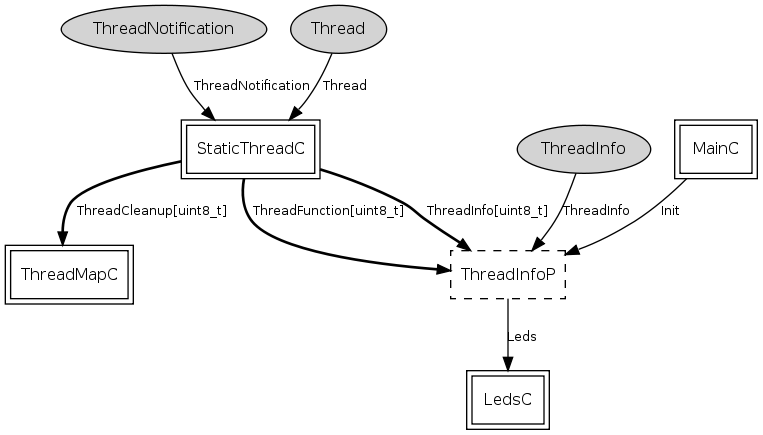
\includegraphics[scale=0.5]{tos-lib-tosthreads-system-ThreadC.png}

\paragraph{\textit{chips/atm128/chip\_thread.h}:}
Antes de expor as funções do escalonador de threads, é importante expor algumas macros de baixo nível que realizam a
troca de contexto. Para guardar o contexto de hardware da thread, criaram a estrutura \textit{thread\_regs\_t}.
\begin{lstlisting}
typedef struct thread_regs {
    uint8_t status;
    uint8_t r0;
    ...
    uint8_t r31;
} thread_regs_t;
\end{lstlisting}
Existem também algumas macros para salvar e restaurar estes registradores.
\begin{lstlisting}
 #define SAVE_STATUS(t)                              \
    __asm__("in %0,__SREG__ \n\t" : "=r" ((t)->regs.status) : );

//Save General Purpose Registers
#define SAVE_GPR(t)                                      \
    __asm__("mov %0,r0 \n\t" : "=r" ((t)->regs.r0) : );  \
    ...

//Save stack pointer
#define SAVE_STACK_PTR(t)             \
    __asm__("in %A0, __SP_L__\n\t"    \
    "in %B0, __SP_H__\n\t"            \
    :"=r"((t)->stack_ptr) : );

#define SAVE_TCB(t) \
   SAVE_GPR(t);      \
   SAVE_STATUS(t);   \
   SAVE_STACK_PTR(t) 

//Definicao das macros de restauracao
...

#define SWITCH_CONTEXTS(from, to) \
   SAVE_TCB(from);                 \
   RESTORE_TCB(to)
\end{lstlisting}
Por último, são definidas duas macros para preparação da thread.
%!!!Ainda não descobri para que serve isso exatamente!!!
%O endereço de uma função será colocado no topo da pilha da thread. Pra que ?
%O status é salvo quando SP está apontando para a pilha da thread atual e não para a pilha da que está sendo preparada.
\begin{lstlisting}
 #define SWAP_STACK_PTR(OLD, NEW) \
   __asm__("in %A0, __SP_L__\n\t in %B0, __SP_H__":"=r"(OLD):);\
   __asm__("out __SP_H__,%B0\n\t out __SP_L__,%A0"::"r"(NEW))
 
#define PREPARE_THREAD(t, thread_ptr)                      \
{  uint16_t temp;                                        \
   SWAP_STACK_PTR(temp, (t)->stack_ptr);                 \
   __asm__("push %A0\n push %B0"::"r"(&(thread_ptr)));   \
   SWAP_STACK_PTR((t)->stack_ptr, temp);                 \
   SAVE_STATUS(t)                                        \
}
\end{lstlisting}

\paragraph{\textit{system/TinyThreadSchedulerP.nc}:}
Durante a inicialização do sistema muitas inicializações são feitas através da interface \textit{Init} amarrada ao
compontente \textit{MainC}. Isso ocorre com a \textit{system/StaticThreadP.nc}. Como visto acima, durante a execução
desta função, o escalonador é chamado através do comando a seguir.
\begin{lstlisting}
command error_t ThreadScheduler.initThread(uint8_t id) {
    thread_t* t = (call ThreadInfo.get[id]());
    t->state = TOSTHREAD_STATE_INACTIVE;
    t->init_block = current_thread->init_block;
    call BitArrayUtils.clrArray(t->joinedOnMe, sizeof(t->joinedOnMe));
    PREPARE_THREAD(t, threadWrapper);
        //uint16_t temp;                                        \
        //SWAP_STACK_PTR(temp, (t)->stack_ptr);                 \
        //__asm__("push %A0\n push %B0"::"r"(&(threadWrapper)));   \
        //SWAP_STACK_PTR((t)->stack_ptr, temp);                 \
        //SAVE_STATUS(t)   
    return SUCCESS;
}
\end{lstlisting}
É importante notar que na macro \textit{PREPARE\_THREAD()}, o endereço da função \textit{threadWrapper} está sendo
empilhado na pilha da thread. Está função encapsula a chamada para a execução da thread.
\begin{lstlisting}
void threadWrapper() __attribute__((naked, noinline)) {
    thread_t* t;
    atomic t = current_thread;

    __nesc_enable_interrupt();
    (*(t->start_ptr))(t->start_arg_ptr);

    atomic {
        stop(t);
        sleepWhileIdle();
        scheduleNextThread();
        restoreThread();
    }
}
\end{lstlisting}

No laço principal do escalonador de tarefas, quando não há mais nada para executar, a thread atual é suspensa. Com isso
o controle é passado para o escalonador de threads através do comando \textit{suspendCurrentThread()}. Na demostração de
código abaixo, algumas chamadas a funções são substituídas pelo seus corpos, para facilitar o entendimento.
\begin{lstlisting}
async command error_t ThreadScheduler.suspendCurrentThread() {
    atomic {
        if(current_thread->state == TOSTHREAD_STATE_ACTIVE) {
            current_thread->state = TOSTHREAD_STATE_SUSPENDED;
            //suspend(current_thread);
            #ifdef TOSTHREADS_TIMER_OPTIMIZATION
                num_runnable_threads--;
                post alarmTask();
            #endif
            sleepWhileIdle();
            //interrupt(current_thread);
            yielding_thread = current_thread;
            //scheduleNextThread();
            if(tos_thread->state == TOSTHREAD_STATE_READY)
                current_thread = tos_thread;
            else
                current_thread = call ThreadQueue.dequeue(&ready_queue);

            current_thread->state = TOSTHREAD_STATE_ACTIVE;
            //fim scheduleNextThread();

            if(current_thread != yielding_thread) {
                //switchThreads();
                void switchThreads() __attribute__((noinline)) {
                    SWITCH_CONTEXTS(yielding_thread, current_thread);
                 }
                //fim switchThreads();
            }
            //fim interrupt(...)
            //fim suspend(current_thread);
            return SUCCESS;
        }
        return FAIL;
    }
}
\end{lstlisting}
É muito importante notar que a função \textit{switchThreads()} não é \textit{inline}. Isso significa que os valores dos
registradores serão empilhados. Haverá então uma troca de contexto e o registrador SP apontará para a pilha da nova
thread. Por último, a função \textit{switchThreads()} retornará para o endereço que está no topo da nova pilha. Este
novo endereço, como visto acima, aponta para a função \textit{threadWrapper()}. Esta por sua vez, através de uma função
e duas sinalizações executa a thread.

%----------------------------------------------------------------------------------------------------
\section{Escalonadores propostos para o TinyOS}\label{escalonadorespropostos}
Nesta seção apresentamos o projeto e as etapas de implementação de novos escalonadores
de tarefas para o TinyOS.
Implementamos três propostas: escalonador EDF (\textit{Earliest Deadline First}), escalonador com prioridades,  
e escalonador multi-nível.

%-----------------------------
\subsection{Escalonador EDF (\textit{Earliest Deadline First})}\label{escalonadoredf}
Este escalonador \footnote{O \cite{TEP106} disponibiliza um protótipo} aceita tarefas com deadline e 
elege aquelas com menor \textit{deadline} para executar. A interface usada para criar
esse tipo de tarefas é \textit{TaskDeadline}. O \textit{deadline} é passado por parâmetro pela função \textit{postTask}.
As tarefas básicas (\textit{TaskBasic}) também são aceitas, como recomendado pelo TEP 106\cite{TEP106}.

Em contraste, o escalonador não segue outra recomendação: não elimina a possibilidade de 
\textit{starvation} pois as tarefas
básicas só são atendidas quando não há nenhuma tarefa com \textit{deadline} esperando para executar. 
A fila de prioridades é implementada da mesma forma que a do escalonador 
padrão\ref{escalonadorpadrao}, a única mudança está na inserção. Para
inserir, a fila é percorrida do começo até o fim, procurando-se o local exato de inserção.
Portanto, o custo de inserir é $\bigcirc(n)$, e o custo de retirar da fila é $\bigcirc(1)$. 
%Uma possível modificação seria utilizar uma \textit{heap}, mudando o custo de inserção  de 
%retirada para $\bigcirc(\logn)$.

%!!!explicar esse trecho melhor depois!!!
%A princípio tive problemas com o componente \textit{Counter32khzC}, 
%pois ele não existe para  a plataforma \textit{micaz}. Para poder compilar o
%escalonador foi preciso retirá-lo. Ele era usado para calcular a hora atual, e somar ao deadline. 
%Sem esse componente, temos um escalonador de prioridades (mínimo). 

%-----------------------------
\subsection{Escalonador com prioridades}\label{escalonadorprioridade}
Desenvolvemos um escalonador onde é possível estabelecer prioridades para as tarefas. 
A prioridade é passada como parâmetro através 
do comando \textit{postTask}. Quanto menor o número passado, maior a preferência da tarefa, sendo 0 a
mais prioritária e 254 a menos prioritária.
As \textit{Tasks} básicas também são aceitas, e são consideradas as tarefas com menor prioridade.

Foram encontrados dois problemas de \textit{starvation}. O primeiro relacionado com as tarefas básicas,
onde elas só seriam atendidas caso não houvesse nenhuma tarefa com prioridade na fila. Para resolver isso, foi definido um
limite máximo de tarefas prioritárias que podem ser atendidas em sequência. Caso esse limite seja excedido, uma tarefa
básica é atendida. O segundo é relacionado às próprias tarefas com prioridade. 
Se entrar constantemente \textit{tasks} com alta
prioridade, é possível que as de baixa prioridade não sejam atendidas. A solução se deu através do envelhecimento de
tarefas. Ou seja, \textit{tasks} que ficam muito tempo na fila, têm sua importância aumentada.

Dois tipos de estrutura de dados foram usadas para a organização das tarefas, uma fila comum e uma \textit{heap}. Com
isso, totalizou-se quatro diferentes versões do escalonador:
\begin{enumerate}
    \item Fila comum sem envelhecimento
    \item Fila comum com envelhecimento
    \item Heap sem envelhecimento
    \item Heap com envelhecimento
\end{enumerate}
A seguir uma tabela com a complexidade de inserção e remoção para cada escalonador:
\begin{center}
    \begin{tabular}{ | l | l | l | l | p{5cm} |}
    \hline
    Escalonador & Inserção & Remoção \\ \hline
    Fila, sem envelhecimento & $\bigcirc(n)$ & $\bigcirc(1)$ \\ \hline 
    Heap, sem envelhecimento & $\bigcirc(\log(n))$ & $\bigcirc(\log(n))$ \\ \hline
    Fila, com envelhecimento & $\bigcirc(n)$ & $\bigcirc(n)$ \\ \hline
    Heap, com envelhecimento & $\bigcirc(\log(n))$ & $\bigcirc(n)$ \\ \hline
    \end{tabular}
\end{center}

%-----------------------------
\subsection{Escalonador multi-nível}
No TinyOS, percebe-se uma divisão clara dos tipos de serviços: 
\begin{description}
    \item[Rádio] Comunicação sem fio entre diferentes nós da rede através de ondas de rádio.
    \item[Sensor] Sensoriamento de diferentes características do ambiente.
    \item[Serial] Comunicação por fio entre um nó e uma estação base (PC).
    \item[Básica] Outros serviços, como por exemplo temporizador.
\end{description}
Por isso, desenvolvemos um escalonador que divide as tarefas de acordo com os tipos definidos acima.
Cada tipo de tarefa tem sua própria fila com política \textit{First-in First-out}, e as filas mais importantes devem ser
atendidas por completo para que as outras sejam antendidas.

%!!!detalhar esse trecho melhor depois!!!
%Definiu-se que a ordem de prioridade seria serial, rádio, sensor e por último básica.

%----------------------------------------------------------------------------------------------------
\section{Experimentos realizados}\label{resultados}
Nesta seção apresentamos os experimentos realizados e os resultados obtidos.

%---------------------------------
\subsection{Experimentos com o escalonador de tarefas padrão}
Antes de começar a desenvolver outros escalonadores de tarefas, foi feito um experimento com o escalonador 
padrão que utiliza a política \textit{First in, First Out}.
Para medir a complexidade na prática, foi desenvolvida uma aplicação de teste. Nela cada tarefa executa um loop de 65000
iterações, fazendo uma simples multiplicação em cada iteração. O número de tarefas variou entre 20, 50 e 100.
Na tabela a seguir pode-se ver o tempo de execução em microsegundos:
\begin{center}
    \begin{tabular}{ | l | l | l | l | p{5cm} |}
    \hline
    Escalonador              & 20 Tarefas & 50 Tarefas & 100 Tarefas \\ \hline
    Escalonador Padrão       & 1366 & 1849 & 2652 \\ \hline
    \end{tabular}
\end{center}

%---------------------------------
\subsection{Experimentos com o escalonador com prioridades}
Para avaliar o desempenho com o escalonador com prioridades foi desenvolvida a mesma aplicação de teste,
onde cada tarefa executa um loop de 65000 iterações, fazendo uma simples multiplicação em cada iteração. 
O número de tarefas variou entre 20, 50 e 100.
Na tabela a seguir pode-se ver o tempo de execução em microsegundos:
\begin{center}
    \begin{tabular}{ | l | l | l | l | p{5cm} |}
    \hline
    Escalonador              & 20 Tarefas & 50 Tarefas & 100 Tarefas \\ \hline
    Escalonador Padrão       & 1366 & 1849 & 2652 \\ \hline 
    Fila, sem envelhecimento & 1733 & 4660 & 13721 \\ \hline 
    Heap, sem envelhecimento & 2603 & 4308 & 7486 \\ \hline
    Fila, com envelhecimento & 2278 & 7887 & 26066 \\ \hline
    Heap, com envelhecimento & 2665 & 4510 & 7887 \\ \hline
    \end{tabular}
\end{center}

Podemos perceber que, para um número pequeno de tarefas, a fila é mais eficiente que a heap. Isso acontece pois
não é compensado o \textit{overhead} do algoritmo da heap.

%----------------------------------------------------------------------------------------------------
\section{Conclusões}\label{conclusoes}
As redes de sensores sem fio podem ser aplicadas em diversas áreas, por exemplo, monitoramento de oscilações 
e movimentos de pontes, observação de vulcões ativos, previsão de incêndio em florestas, entre outras. 
Muitas dessas aplicações podem atingir alta complexidade, exigindo a construção de algoritmos robustos, 
como roteamento de pacotes diferenciado.
Os escalonadores desenvolvidos neste trabalho poderão ajudar os desenvolvedores dessas aplicações complexas,
oferecendo maior flexibilidade no projeto das soluções, como, por exemplo, 
a possibilidade de priorizar certas atividades da aplicação (comunicação via rádio ou serial, sensoriamento, etc.).
Porém é preciso analisar se o ganho em flexibilidade, oferecido pelo escalonador, irá compensar o
\textit{overhead} gerado.
Pretendemos realizar ainda outros experimentos com os escalonadores desenvolvidos, considerando diferentes
tipos de aplicações. 

Sem um fluxo contínuo de execução, sobre a perspectiva do programador, as aplicações grandes ficam difíceis de
implementar e entender. O modelo de \textit{threads} oferecido no 
TinyOS 2.1.X\cite{TEP134} facilita este problema. Entretanto, por ser um modelo preemptivo, o custo de
gerência das threads pode implicar em queda de desempenho das aplicações. 
Com a implementação de um mecanismo de cooperação baseado em co-rotinas pretendemos
oferecer uma alternativa a mais para o programador.


\subsection{Atividades extras}
Outras atividades realizadas pelo aluno foram:
\begin{itemize}
    \item Participação no evento SBAC-PAD 2010 -- 
{\em 22nd International Symposium on Computer Architecture and High Performance Computing}.
    \item Participação no minicurso 
{\em Redes de sensores sem fio sob a perspectiva do EPOS}~\cite{HoellerFrohlich/10}, 
apresentado no SBAC-PAD 2010.    
    \item Participação em seminário do grupo de Redes de Computadores e Sistemas Distribuídos (RCSD)
do Programa de Pós-Graduação em Informática (PPGI).
\end{itemize}

\subsection{Avaliação do Bolsista}
A iniciação científica está sendo uma ótima oportunidade para etender como funciona uma pesquisa. Por meio desse trabalho pude conhecer as redes de sensores sem fio, e um sistema operacional diferente dos convêncionais. É muito prazeroso poder, ao mesmo tempo, estudar e desenvolver novidades. Foi interessante perceber que na prática temos de tomar cuidado com questões que às vezes na teoria são deixadas de lado. Por exemplo, o caso do \textit{overhead} no algoritmo de \textit{Heap} dos escalonadores. 

Este trabalho ajudou na minha decisão de seguir carreira acadêmica. Ainda estou tendo a oportunidade de pesquisar em uma área pouco explorada no meu deparatamento.

%----------------------------------------------------------------------------------------------------
%\bibliographystyle{alpha}
\bibliographystyle{unsrt}
\bibliography{ic}
\end{document}
